\documentclass[t, 11pt]{beamer}
\pdfmapfile{+sansmathaccent.map}
%%% Работа с русским языком
\usepackage{cmap}				
\usepackage{mathtext} 				
\usepackage[T2A]{fontenc}		
\usepackage[utf8]{inputenc}			
\usepackage[english,russian]{babel}	

\usetheme{Ilmenau}
\usecolortheme{lily} % Цветовая схема



%%% Работа с картинками
\usepackage{graphicx}

\usepackage{csquotes}

\hypersetup{				
	colorlinks=true,       	
	linkcolor=blue,          
	citecolor=blue,       
	filecolor=magenta,      
	urlcolor=magenta           
}


\title{Scrapping}
\subtitle{Internet rvest selenium \\ web technologies}
\author{Чувакин Сергей}
\date{\today}
%\institute[<<Анализ больших данных в бизнесе, экономике и обществе>>]{<<Высшая школа экономики>>}
\institute{R meetup}
\begin{document}
	\frame[plain]{\titlepage}
%	\section{Outline}
%	
%	\begin{frame}
%		\frametitle{\insertsection} 
%		\begin{block} {}
%			 
%			\hyperlink{l1}{\beamerbutton{Language models}}
%		\end{block}
%			\begin{block}{}
%		\hyperlink{l2}{\beamerbutton{Probabalistic}}
%		\end{block}
%				\begin{block}{}
%		\hyperlink{l2}{\beamerbutton{Perplexity}}
%		\end{block}
%	\end{frame}
%	

\subsection{Internet}
\begin{frame}
	\frametitle{\insertsection}
	\frametitle{\insertsubsection}  
		WWW vs. Internet ?
\end{frame}

\begin{frame}
	\frametitle{\insertsection}
	\frametitle{\insertsubsection}  
	\begin{itemize}
		\item Серверы 
		\item Клиенты
		\item Третья сторона...
	\end{itemize}
\end{frame}

\section{Structure}
\subsection{HTML\\CSS}
\begin{frame}
	\frametitle{\insertsection}
	\frametitle{\insertsubsection}  
	HTML - язык разметки, который отвечает за содержание страницы. 
	
	
	CSS - язык стилей, который отвечает, за то, как будет выглядеть страница.  

\end{frame}


\begin{frame}
	\frametitle{\insertsection}
	\frametitle{\insertsubsection} 
	Пример: 
... 
\end{frame}


\section{web queries}

\begin{frame}
	\frametitle{\insertsection}
	\frametitle{\insertsubsection}  
	Интернет запрос - структурированная конструкция позволяющая получать содержимое страниц с удаленных серверов. 
	
	Сценарий: request - response. 
\begin{itemize}
	\item headers
	\item body
	\item cookies
	\item data 
	\item parameters (params)
	\item cache
	\end{itemize}
\end{frame}


\subsection{headers}

\begin{frame}
	\frametitle{\insertsection}
	\frametitle{\insertsubsection}  
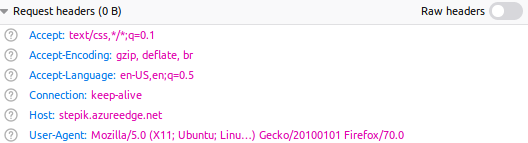
\includegraphics[width=0.8\linewidth]{head.png}
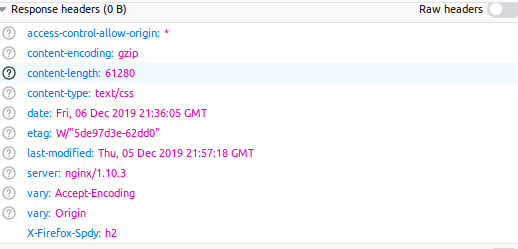
\includegraphics[width=0.8\linewidth]{head_res.png}
\end{frame}

\subsection{body}

\begin{frame}
	\frametitle{\insertsection}
	\frametitle{\insertsubsection}  
	Методы: 
	\begin{itemize}
		\item GET
		\item HEAD
		\item POST
		\item PUT 
		\item PATCH
		\item DELETE
		\item etc
	\end{itemize}
	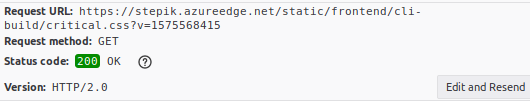
\includegraphics[width=0.8\linewidth]{req.png}
\end{frame}

\subsection{cookies}

\begin{frame}
	\frametitle{\insertsection}
	\frametitle{\insertsubsection}  
	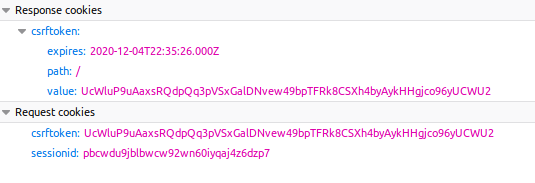
\includegraphics[width=0.8\linewidth]{cook.png}
\end{frame}


\subsection{params}

\begin{frame}
	\frametitle{\insertsection}
	\frametitle{\insertsubsection}  
	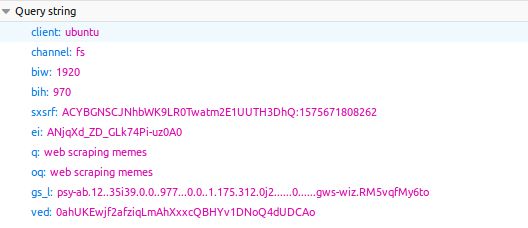
\includegraphics[width=0.8\linewidth]{params.png}
\end{frame}


\subsection{Cache}

\begin{frame}
	\frametitle{\insertsection}
	\frametitle{\insertsubsection}  
	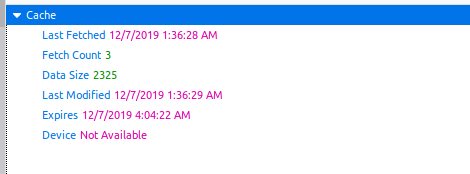
\includegraphics[width=0.8\linewidth]{cach.png}
\end{frame}


\subsection{Что еще?}

\begin{frame}
	\frametitle{\insertsection}
	\frametitle{\insertsubsection}  
	\begin{itemize}
	\item Протоколы 
	\item Архитектура DOM
	\item MVC фреймворки 
	\item frontend-backend 
	\item Sessions 	
	\item Работа с СУБД 
	\item etc
\end{itemize}
\end{frame}


\subsection{AJAX}

\begin{frame}
	\frametitle{\insertsection}
	\frametitle{\insertsubsection}  
	AJAX - технология верстки страниц с помощью ЯП (java script).
	
	\vspace{0.5cm}
	
	
\includegraphics[width=0.5\linewidth]{ajax_mem.jpg}
	
	пример - http://zpp.rospotrebnadzor.ru/Forum/Appeals
\end{frame}


\subsection{proxy}

\begin{frame}
	\frametitle{\insertsection}
	\frametitle{\insertsubsection}  
	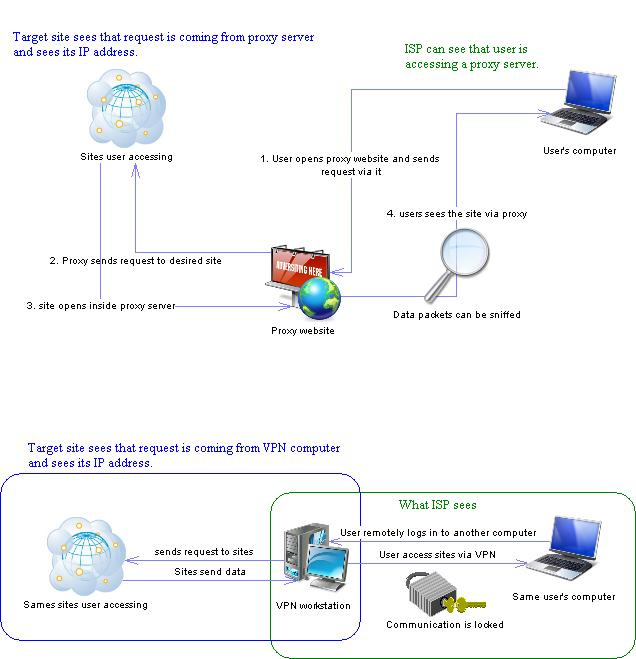
\includegraphics[width=0.8\linewidth]{proxy.jpg}
\end{frame}

\subsection{vpn}

\begin{frame}
	\frametitle{\insertsection}
	\frametitle{\insertsubsection}  
	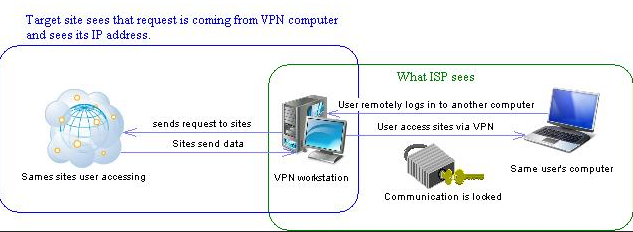
\includegraphics[width=0.8\linewidth]{vpn.png}
\end{frame}
%	\begin{frame}
%	\frametitle{\insertsection}
%	\frametitle{\insertsubsection}  
%	Синонимы кватификаторов 
%	\begin{center}
%		\begin{table}[]
%			\begin{tabular}{c|c|c}
%				\hline
%				Синоним &Расшифровка &Квантификатор \\
%				\hline
%		+ & 1 и более раз &\{1,\}   \\
%		* & 0 и более раз &\{0,\}   \\
%
%		? &  0 или 1 раз& \{0,1\}  \\
%  
%			\end{tabular}
%		\end{table}
%	\end{center}
%\end{frame}

%\begin{frame}
%	\frametitle{\insertsection}
%	\frametitle{\insertsubsection}  
%	Чтобы убрать жаность необходимо добавить ?
%	
%	\vspace{0.5cm}
%	
%	Строка на вход  <<( dfghvb ) sdvsd ( sdcvkjnh ) sdvsd ( dkjhvgr ) sdvfv.>>
%	
%	\vspace{0.5cm}
%	
%	шаблон: r"$\backslash$(.+?$\backslash$)"
%	
%	\vspace{0.5cm}
%	
%	на выходе: ['dfghvb', 'sdcvkjnh', 'dkjhvgr']
%	
%\end{frame}



%	\begin{frame}
%	\frametitle{\insertsection}
%	\frametitle{\insertsubsection}
%	
%	
%	\vspace{1cm}
%	\includegraphics[width=0.9\linewidth]{page2.png}
%	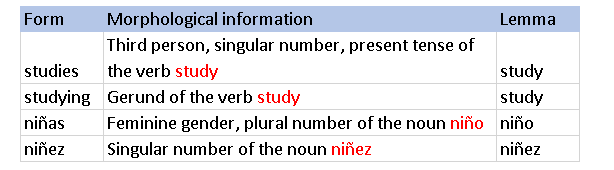
\includegraphics[width=0.7\linewidth]{lem.png}
%\end{frame}
\end{document}